\documentclass[10pt]{article}
\usepackage[a4paper,bottom=3cm]{geometry}
\usepackage[english]{babel}
\usepackage[utf8]{inputenc}
\usepackage{amsmath}
\usepackage{amssymb}
\usepackage{graphicx}
\usepackage{subfig}
\usepackage{hyperref}

\author{Takudzwa Togarepi, Julian Bopp }
\title{Project Part 1: Probabilistic modeling of the femur anatomy}
\begin{document}

\maketitle
\begin{abstract}
\noindent
The femur bone is a crucial part of the human anatomy used in forensic science due to its size and strength. It can provide valuable insights into the gender and geographical origin of the person whose remains are being analyzed. This is because femurs of people with similar geographical origin or of the same gender tend to be similar. However it is likely that when examining human remains we only get a partial or deformed femur, this is where we would need femur reconstruction to model what the full femur would have looked like and analyze it. In this project we came up with a model which we would use to reconstruct given partial femurs. We also analyzed and validated our model using statistical approaches.\\

\noindent
$\bold{Keywords}$: femur, forensics, gender determination, reconstruction, modeling.
\end{abstract}

\section{Introduction}
The main goal of this project is to develop a probabilistic shape model for femur bones which is used to reconstruct partial femurs.
Femur bone reconstruction is an important task in the field of forensics as it can aid in the human identification just by analyzing the femur bones from the human remains . In this paper, we present an approach to develop a probabilistic shape model for femur bones using a combination of rigid alignment, Gaussian Process modeling, Iterative Closest Points (ICP), and Principal Component Analysis(PCA).\\

\noindent
In our approach we used a dataset of femur meshes and femur landmarks, comprising 47 samples each. We first applied rigid alignment, followed by building a Gaussian Process model(GP-model) to capture the shape variation of the femur bones. We then used an iterative alignment refinement technique called ICP to fit the GP-model by aligning the femur meshes with the model.\\

\noindent
After implementing ICP, we built a PCA model to reduce the dimensionality of the data and speed up the reconstruction process. 





\section{Methods}
\subsection{Rigid Alignment}
\subsection{GP model}
\subsection{ICP}
\subsection{PCA}


In this section you can describe the methods you used to solve the problem.

\newpage
\section{Experiments and results}
\subsection{Data and experimental setup}

%Explain the data with which you are experimenting.
%Highlight aspects of the data that are particularly interesting
%for the project.

The data on which we are experimenting consists of 46 femurs. Included in this data are landmarks $L0,\dots,L5$ for every femur.
In particular $L3,L4$, as seen in figure \ref{fig:landmark_width}, can be used to estimate the width of the femur, whereas $L2,L5$, as seen in figure \ref{fig:landmark_length}, can be used to estimate the length.

\begin{figure}[h]
\centering
\includegraphics[scale=0.2]{screenshots/L3blue_L4red_width.png}
\caption{Landmark $L3$ in blue, and landmark $L4$ in red. Used to estimate width of the femur bone.}
\label{fig:landmark_width}
\end{figure}

\begin{figure}[h]
\centering
\includegraphics[scale=0.2]{screenshots/L2red_L5green_length.png}
\caption{Landmark $L3$ in blue, and landmark $L4$ in red. Used to estimate length of the femur bone.}
\label{fig:landmark_length}
\end{figure}
\noindent
To estimate the length of a femur we calculate the distance between the $L2$ and $L5$ landmark, similarly we estimate the width by calculating the distance between the $L3$ and $L4$ landmark. We display the measurements made from the 46 femurs in figure \ref{fig:scatterplot_femurdata} and summarize them in table \ref{table:mean_variance_femur_data} by calculating the mean and variance.
\begin{figure}
\centering
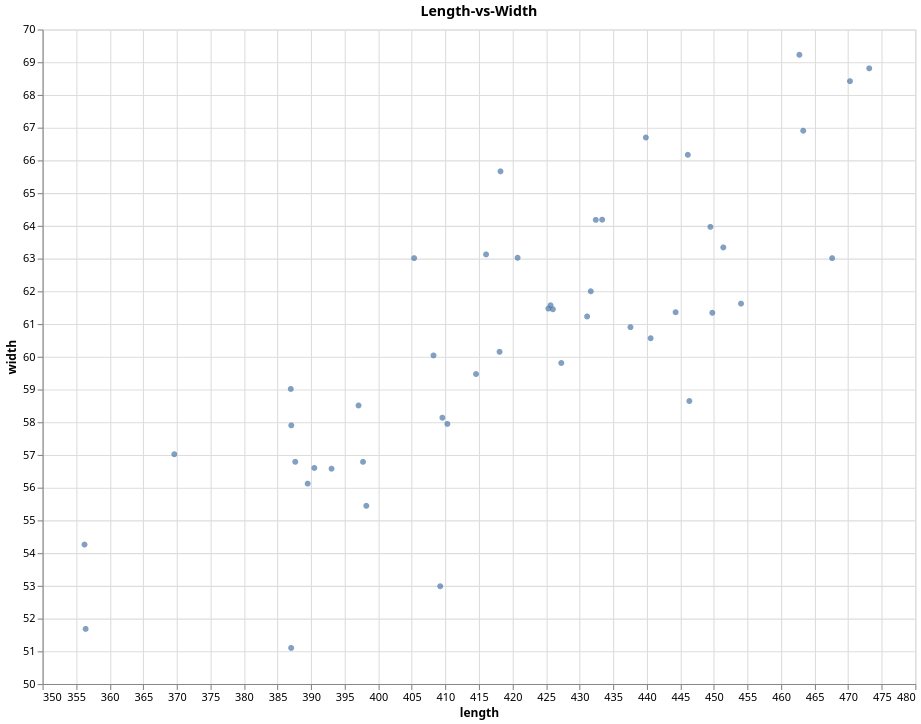
\includegraphics[scale=0.4]{screenshots/femur_data_length_width_scatter.png}
\caption{Scatterplot of calculated length and width of the femur data}
\label{fig:scatterplot_femurdata}
\end{figure}

\begin{table}[h!]
\centering
\begin{tabular}{c|r|r}
 & Mean & Variance \\
\hline
Length & 420.80 & 841.94 \\
Width & 60.61 & 18.13
\end{tabular}
\caption{Mean and variance of length and width of the femur data.}
\label{table:mean_variance_femur_data}
\end{table}

\noindent
We notice a high variability of the data. This gives reason to believe that the 46 femur samples are not from subjects that all share similar femurs. More precisely, the data probably originates from males and females with a large variability in height, and therefore, a large variability in femur length and width. Visually, figure \ref{fig:scatterplot_femurdata} gives reason to believe that the length and width are correlated. There is a trend that shows that an increase in length comes with an increase in width.




% Side by Side picture mode
%\begin{figure}%
%    \centering
%    \subfloat[\centering label 1]{{\includegraphics[width=5cm]{../screenshots/L3blue_L4red_width.png} }}%
%    \qquad
%    \subfloat[\centering label 2]{{\includegraphics[width=5cm]{../screenshots/L2red_L5green_length.png} }}%
%    \caption{2 Figures side by side}%
%    \label{fig:example}%
%\end{figure}

\newpage
\subsection{Experimental results}

\newpage
\section{Conclusion}

Add your conclusion here. What is the main result? What did you achieve, what 
needs to be done. 


\end{document}
